% Template for Cogsci submission with R Markdown

% Stuff changed from original Markdown PLOS Template
\documentclass[10pt, letterpaper]{article}

\usepackage{cogsci}
\usepackage{pslatex}
\usepackage{float}
\usepackage{caption}

% amsmath package, useful for mathematical formulas
\usepackage{amsmath}

% amssymb package, useful for mathematical symbols
\usepackage{amssymb}

% hyperref package, useful for hyperlinks
\usepackage{hyperref}

% graphicx package, useful for including eps and pdf graphics
% include graphics with the command \includegraphics
\usepackage{graphicx}

% Sweave(-like)
\usepackage{fancyvrb}
\DefineVerbatimEnvironment{Sinput}{Verbatim}{fontshape=sl}
\DefineVerbatimEnvironment{Soutput}{Verbatim}{}
\DefineVerbatimEnvironment{Scode}{Verbatim}{fontshape=sl}
\newenvironment{Schunk}{}{}
\DefineVerbatimEnvironment{Code}{Verbatim}{}
\DefineVerbatimEnvironment{CodeInput}{Verbatim}{fontshape=sl}
\DefineVerbatimEnvironment{CodeOutput}{Verbatim}{}
\newenvironment{CodeChunk}{}{}

% cite package, to clean up citations in the main text. Do not remove.
\usepackage{apacite}

% KM added 1/4/18 to allow control of blind submission


\usepackage{color}

% Use doublespacing - comment out for single spacing
%\usepackage{setspace}
%\doublespacing


% % Text layout
% \topmargin 0.0cm
% \oddsidemargin 0.5cm
% \evensidemargin 0.5cm
% \textwidth 16cm
% \textheight 21cm

\title{Parents Calibrate Speech to Children's Vocabulary Knowledge}


\author{Ashley Leung, Alexandra Tunkel, and Daniel Yurovsky \\
        \texttt{\{ashleyleung, aetunkel, yurovsky\}@uchicago.edu} \\
       Department of Psychology \\ University of Chicago}

\begin{document}

\maketitle

\begin{abstract}
Young children acquire language at rapid rates, and the proposed
mechanisms for learning have focused on children's unique ability to
harvest information from their environments. However, language
development is not simply absorbing input- language is social in nature.
The communicative intent and interactive nature of language must not be
ignored when considering how parental input influences children's
language development. Indeed, studies have shown that parental
responsiveness shapes young children's language learning. Parental
sensitivity (to children's knowledge, intent, etc.) may thus be a better
predictor of children's language development than mere quantity of
speech. The present study examined whether parents calibrate speech to
their children's knowledge in an interactive game. Our results show that
parents modify their language according to beliefs about their
children's vocabulary knowledge, using longer sentences when describing
unfamiliar objects, and shorter sentences for familiar objects.

\textbf{Keywords:}
parent-child interaction; language development; communication
\end{abstract}

\hypertarget{introduction}{%
\section{Introduction}\label{introduction}}

Children learn language at astonishing rates, acquiring thousands of
words by the time they are toddlers. How do children learn so many words
even before they know how to dress themselves? One account for
children's rapid language acquisition is statistical learning. Young
children can attend to the distributional structure of language,
learning to discriminate words and identify word order from speech
streams (Saffran, 2003; Saffran, Aslin, \& Newport, 1996). Statistical
learning can be a powerful tool for early language learning, and
showcases the ability that children have to harvest information from
their surroundings. However, children's language environments may also
play a role in supporting language development.

The way we speak to children often differs from the way we speak to
adults. Child-directed speech (CDS) exists across cultures, and is
characterized by higher pitches and exaggerated enunciations (Cooper \&
Aslin, 1990; Grieser \& Kuhl, 1988). Not only do children prefer CDS
over adult-directed speech (ADS), CDS is also more helpful for language
learning than overheard ADS (Shneidman, Arroyo, Levine, \&
Goldin-Meadow, 2013). One reason why CDS may facilitate language
development is that its structural qualities make speech segmentation
and word learning easier (Thiessen, Hill, \& Saffran, 2005; Yurovsky,
Yu, \& Smith, 2012). It is thus clear that children hear specific types
of input that are facilitative for early language learning.

Children's language environments are not only uniquely suited for their
abilities, but these environments change across development. Parents use
simpler and more redundant language when talking to toddlers, and more
complex syntactic structures when speaking with school-aged children
(Snow, 1972). Importantly, sensitive modification of parent response has
been shown to facilitate learning in children (Hoff-Ginsberg \& Shatz,
1982; Tamis-LeMonda, Kuchirko, \& Song, 2014). The fact that parents
play a role in changing children's language environment, and that
sensitivity to developmental level influences learning point to the
importance of understanding the reason parents change the way they talk
over time.

Why do parents modify the way they speak according to their children?
One possible explanation is that parents are actively teaching their
children. Indeed, some have posited that CDS is an ostensive cue for
social learning, and that infants are born prepared to attend to these
cues (Csibra \& Gergely, 2009). While it may be true that parents hope
to impart knowledge to their children, we argue that effective
communication is the proximal goal. The field of linguistics has long
established that adults communicate in ways that are efficient. For
example, Grice's (1975) maxim of quantity states that speech should be
as informative as necessary, and no more. Adults are able to adhere to
these maxims, adapting speech according to conversational partners'
knowledge as needed for successful communication (Clark \& Wilkes-gibbs,
1986). We argue that the parent's goal to communicate with their child
drives the change in language use.

As parents seek to communicate with their children, they modify their
language as a means to achieve successful communication. Parents use
simpler language and are more linguistically aligned with their younger
children, and these patterns of speech change as their children develop
(Snow, 1972; Yurovsky, Doyle, \& Frank, 2016). Parents are also
sensitive to children's vocabulary knowledge, and the way they refer to
objects change markedly depending on whether they are novel,
comprehended, or familiar to their children (Masur, 1997). The change in
parent speech may indicate adaptations that are aimed at fulfilling the
goal of effective communication, and the language necessary to fulfill
that goal changes as children develop.

Based on work by Masur (1997), we developed a study to investigate how
parents adapt their speech according to their children's vocabulary
knowledge. Masur's study involved parents and children engaging in
unstructured free play, and parents were asked to report children's
vocabulary knowledge after the session. While experimental manipulation
is not completely possible while also eliciting natural speech, our
paradigm allows for more experimental control, and introducing a
communicative goal within a game setting also allows parent utterances
to be more comparable across parent-child dyads. We designed an
interactive iPad game where parents guide their children to select a
particular animal on the iPad. We predicted that parents would modify
their speech based on their beliefs about their children's vocabulary
knowledge. Specifically, we predicted: (1) Parents should use shorter
sentences when describing animals that they believe their children know,
and (2) Upon the second appearance of an animal, parents would adapt the
length of their sentence according to whether the child responded
accurately on the first appearance of the animal.

\hypertarget{method}{%
\section{Method}\label{method}}

\hypertarget{participants}{%
\subsection{Participants}\label{participants}}

Children from age 2;0 to 2;6 and their parents were recruited from a
databse of families in the local community or approached on the floor of
a local science museum in order to achieve a planned sample of 40
parent-child dyads. A total of 45 parent-child pairs were recruited, but
data from five pairs was dropped from analysis due to experimental error
or failure to complete the study. The 40 children \textbf{D DEMOGRAPHICS
HERE}

\hypertarget{stimuli}{%
\subsection{Stimuli}\label{stimuli}}

Eighteen animal images selected from Rossion \& Pourtois (2004) image
set, which is a colored version of the Snodgrass \& Vanderwart (1980)
object set. Animals were selected based on age of acquisition (AoA),
using data from WordBank (Frank, Braginsky, Yurovsky, \& Marchman,
2017). Half of the selected animals had lower AoA (12-20 months), and
the other half had higher AoA (25-31 months).

A modified version of the MacArthur-Bates Communicative Development
Inventory (CDI; Fenson et al., 2007), a parent-reported measure of
children's vocabulary, was administered via an online survey. The
selected animal words were embedded among the \textbf{AMOUNT} words in
the survey. Parents were invited to complete the survey prior to
participating in the study. Two of the animal words--one in the early
AOA and one in the late AOA category were excluded by accident, and so
trials for those words were not included in analysis.

\hypertarget{design-and-procedure}{%
\subsection{Design and Procedure}\label{design-and-procedure}}

Each parent-child pair played an interactive game on iPads. Children
were given two warm-up trials to get used to tapping on an iPad. The
practice and experiment trials began after the warm-up. On each trial,
three images were displayed side by side on the child's screen, and a
single word appeared on the parent's screen (Figure \ref{fig:ipads}).
Parents were instructed to communicate as they normally would with their
child, and encourage them to choose the object corresponding to the word
on their screen. The child was instructed to listen to their parent for
cues. Once an animal was tapped, the trial ended, and a new trial began.
There were a total of 36 experiment trials, such that each animal
appeared as the target twice. Trials were randomized for each
participant, with the constraint that the same animal could not be the
target twice in a row. Practice trials followed the same format as
experimental trials, with the exception that images of fruit and
vegetables were shown. All sessions were videotaped for transcription
and coding.

\begin{CodeChunk}
\begin{figure}[tb]

{\centering 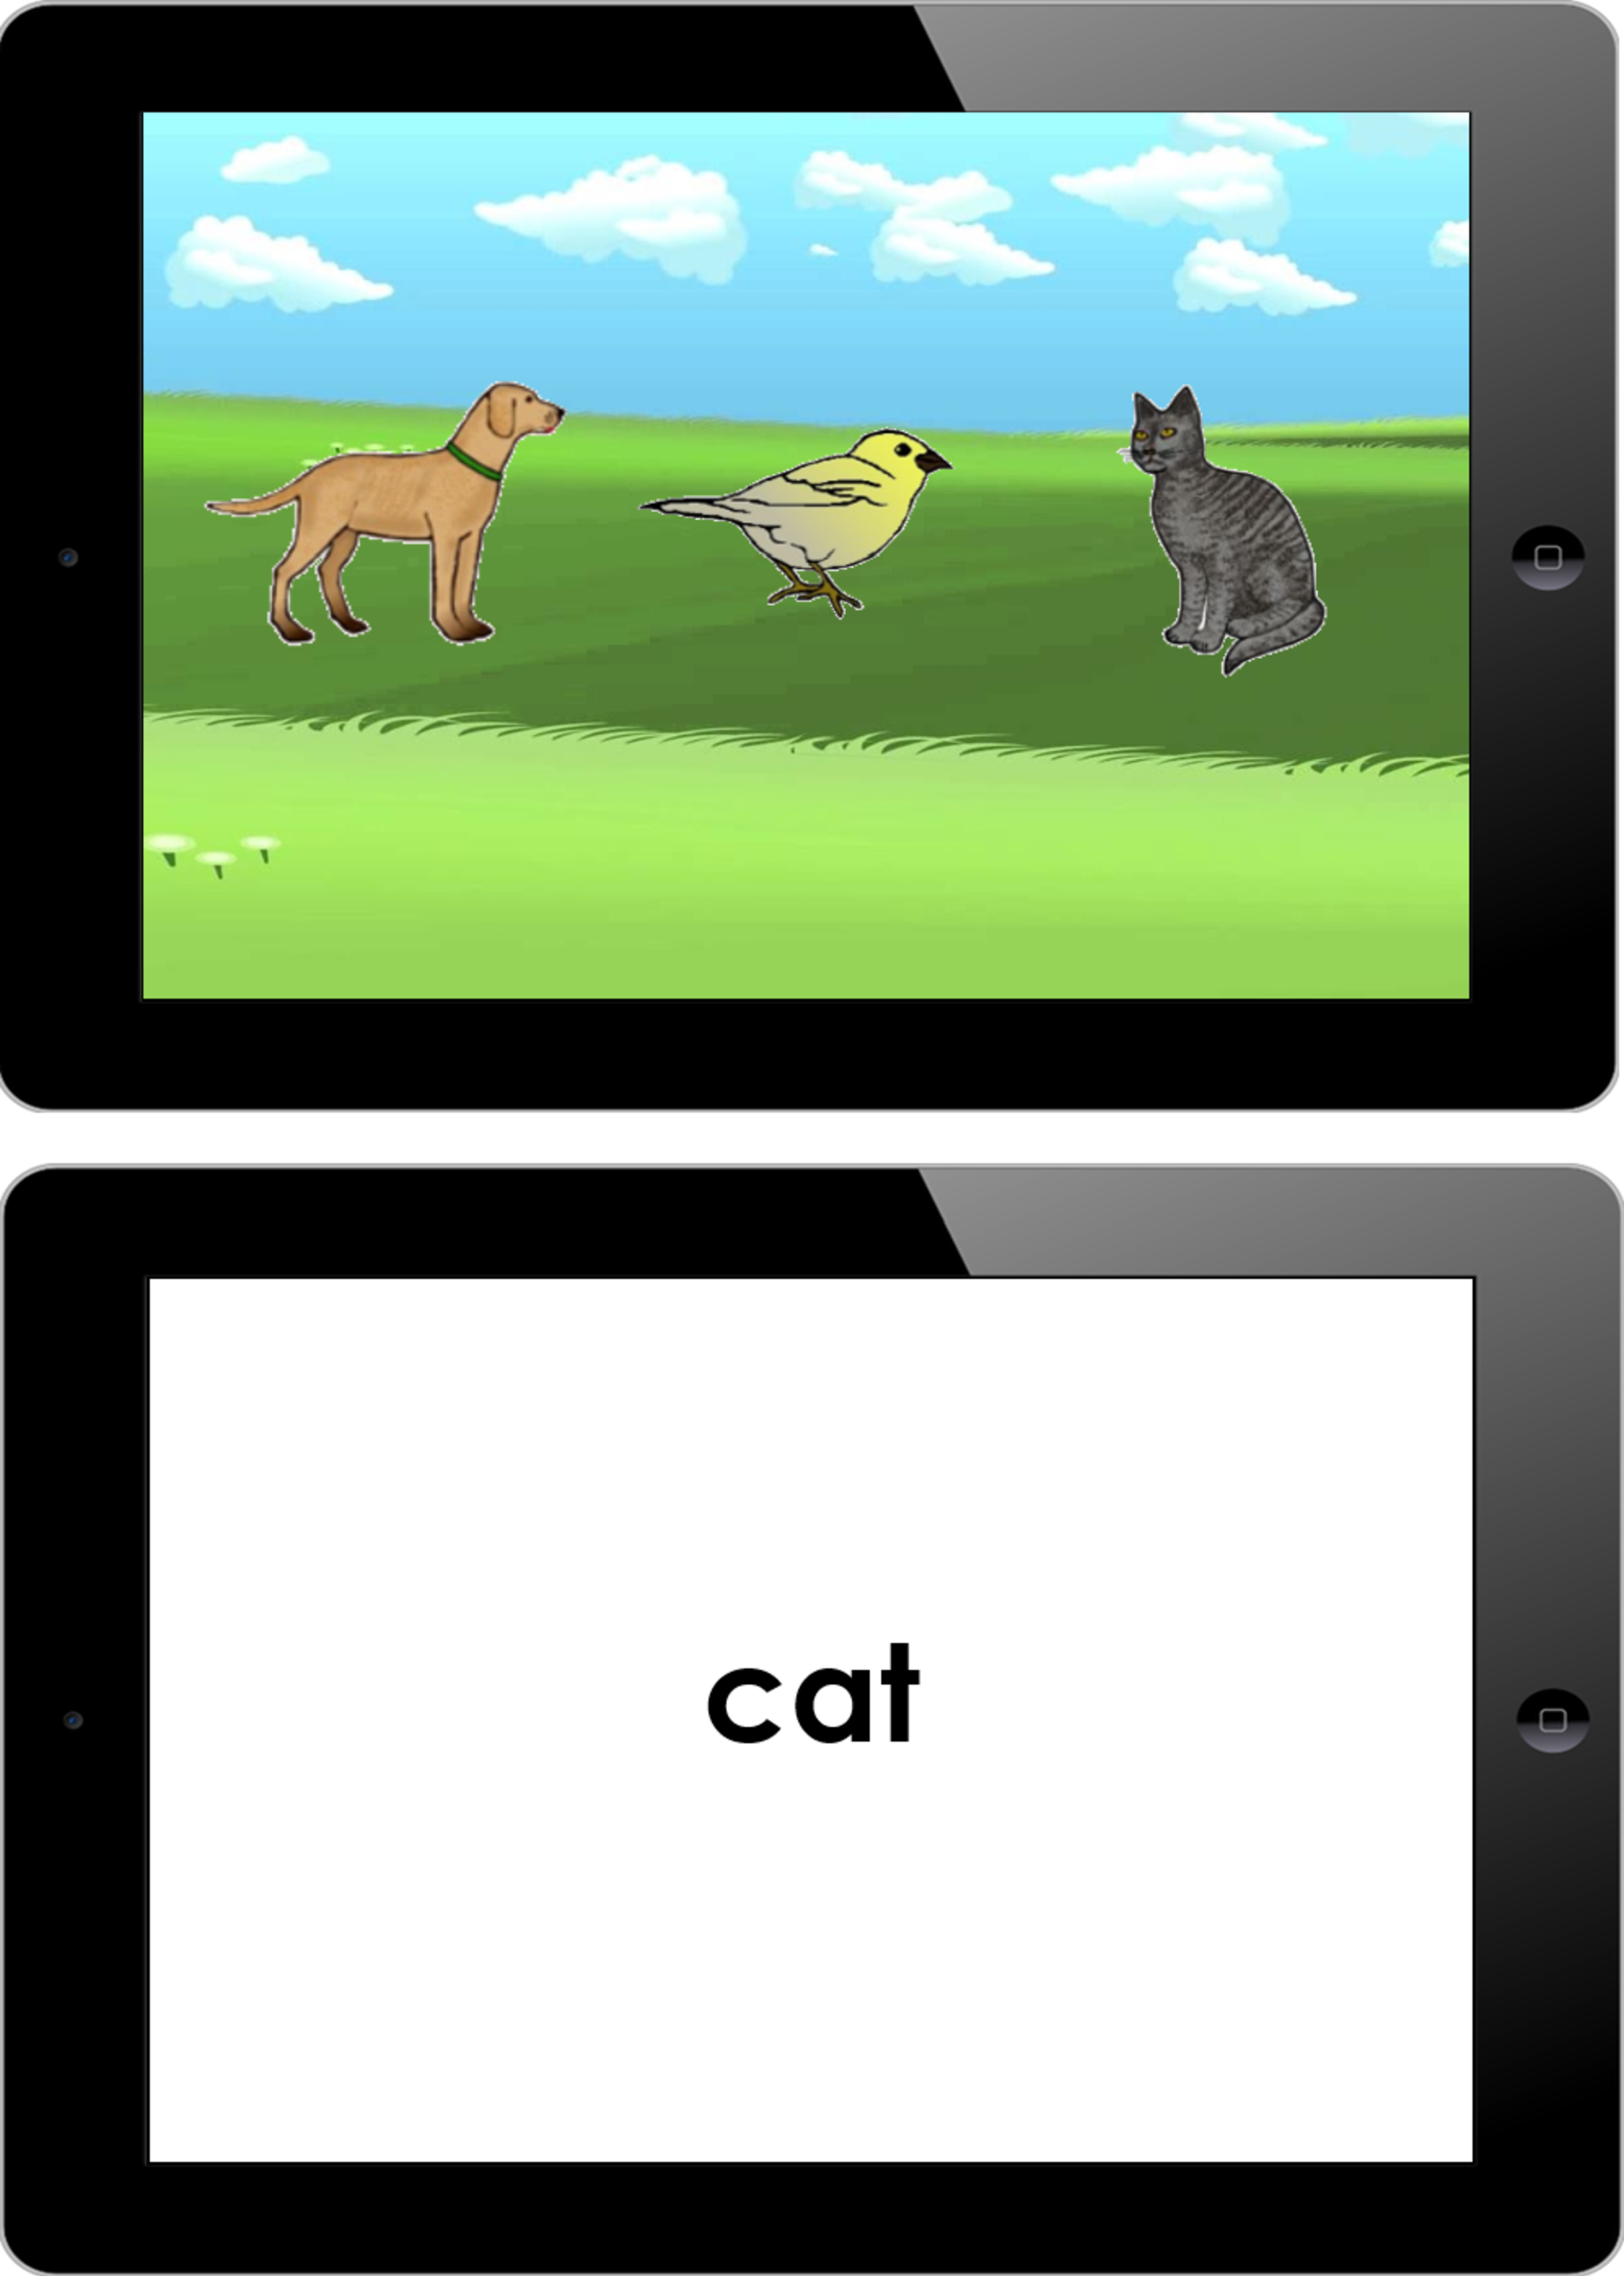
\includegraphics[width=200px]{figs/ipads} 

}

\caption[Example iPad screens for the child (top) and parent (bottom) during the experiment]{Example iPad screens for the child (top) and parent (bottom) during the experiment.}\label{fig:ipads}
\end{figure}
\end{CodeChunk}

\hypertarget{results}{%
\subsection{Results}\label{results}}

The data of interest in this study were parent utterances used during
the interactive game, and parents' responses on the CDI. Transcripts of
the videos were analyzed for utterance length. Parent utterances
irrelevant to the iPad game (e.g.~asking the child to sit down) were not
analyzed. Children's utterances were coded when audible, but were not
analyzed.

\hypertarget{word-difficulty}{%
\subsubsection{Word difficulty}\label{word-difficulty}}

We first confirm that the animals predicted be later learned were less
likely to be marked known by the parents of children in our studies.
Analyses confirmed that animals in the early AoA category were judged to
be understood by 93\% of parents, and items in the late AoA category
were judged understood by 35\%.

\begin{CodeChunk}
\begin{figure}[tb]
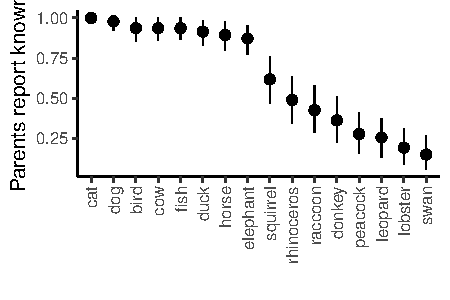
\includegraphics{figs/difficulty_fig-1} \caption[Word difficulties]{Word difficulties.}\label{fig:difficulty_fig}
\end{figure}
\end{CodeChunk}

The difference between these groups was confirmed statistically with a
logistic mixed effects regression with a fixed effect of AoA type and
random effects of participants. The late AoA items were judged known by
a significantly smaller proportion of parents (\(\beta =\) -5.49,
\(t =\) -11.22, \(p\) \textless{} .001). Parents' judgments for each
target word are shown in Figure \ref{fig:difficulty_fig}.

\hypertarget{utterance-length}{%
\subsubsection{Utterance length}\label{utterance-length}}

Utterance length was analyzed in relation to parents' beliefs about
their children's knowledge. Figure 3 shows parents' utterance lengths
for animals that they believe their children know versus those they
believe their children do not know. In line with our prediction, parents
used significantly shorter utterances when talking about animals that
they believe their children know.

In order to examine whether parents modify their speech behaviors within
the timeframe of the experiment, we compared utterance lengths between
first and second appearances of each target. Overall, utterances were
shorter for the second appearance of a given target (Fig. 4).

We also asked whether parents changed their behaviors according to their
children's responses during the game. When accounting for children's
accuracy, we found that parents used longer utterances when their child
responded incorrectly on the first appearance of a target that they
believe their children know. However, no difference in utterance length
was found for words that parents believed their children did not know
(Fig. 5). These results are partially in line with our prediction that
parents would modify their speech during the game.

We did not make specific predictions about accuracy, but our results
show that children performed significantly above chance for both high
and low AoA words (plot coming soon!). A linear model predicting
children's response accuracy found that utterance length, parent belief
about children's knowledge, and the interaction between these two
factors were reliable predictors (Table 1). Specifically, children were
more likely to be correct on trials where parents used longer
utterances. On trials where parents believe their children know the
word, children were more likely to be correct. Finally, there was an
interaction between utterance length and parent belief. Longer
utterances were more likely to be associated with a correct response on
trials where parents believe their children do not know the word.

\hypertarget{discussion}{%
\section{Discussion}\label{discussion}}

Our results indicate that parents speak differently depending on their
beliefs about their children's vocabulary knowledge. Specifically,
parents use shorter sentences when talking about animals that they
believe their children know. Since parents completed the CDI prior to
participating in our study, our data allow us to correlate parent
beliefs and their behaviors. A conceptually similar observational study
by Masur (1997) asked parents to indicate children's vocabulary
knowledge after the observational sessions. While their results also
show that parents' speech differ for familiar and unfamiliar animals, it
is unclear whether parents used children's responses during each session
to assess children's knowledge. Our results not only corroborate their
findings, but allows us to argue that parents' prior beliefs about their
children's knowledge predicts the way they will talk.

Contrary to our predictions, parents did not consistently modify their
speech depending on their children's response. Specifically, utterance
length remained the same for words that parents think their children do
not know, regardless of whether their children responded correctly. This
may indicate that parent sensitivity does not emerge within the short
time frame of a game. However, qualitative analysis of our transcripts
may reveal more about parent behaviors in the case of unfamiliar words.
Utterance length remains relatively long across the first and second
appearance of these animals (see Fig. 5). It is possible that parents
believe their children's accuracy was due to their sufficient
description of the animal (e.g. ``the one that looks like a cat'' for
leopard).

Overall, children performed significantly above change across all
trials. This finding may seem surprising at first glance, given our CDI
data (see Fig. 2). While our results could indicate that parents are
inaccurate in their estimation of children's vocabulary knowledge,
previous studies have found the CDI to be a valid measure of children's
vocabulary (Dale, Bates, Reznick, \& Morisset, 1989). What the high
accuracy may instead reflect is that parents succeeded in their goal to
communicate. Taken together with our finding that parents used longer
sentences for words they think their children do not know, our results
suggest that parents modified their speech as a means to communicate.

One account for explaining our results is that communicative efficiency
is driving parent behavior. Our results suggest that parents may be
adhering Gricean conversational maxims when communicating with their
children, using longer sentences for unfamiliar words, presumably
because more information is necessary in cases where children do not
know the target word. Our study analyzed utterance length as a proxy for
information, but further qualitative analysis will be needed to
determine whether longer utterances do indeed contain more information
(rather than simply consisting of repeated words).

Our results can also be interpreted from a different perspective, in
terms of speaker-design and listener- design theories. Proponents of
speaker-design accounts argue that the speaker's own cognitive
capacities, such as memory retrieval, influences the speech they produce
(MacDonald, 2013). On the other hand, those supporting listener-design
accounts argue that the listener's needs, such as their knowledge level,
drives speaker's language (Jaeger, 2013). The opposing forces driving
communication can be understood as the pressure to produce speech
quickly within a communicative exchange (speaker-design), versus the
pressure to produce speech that is understood by the partner
(listener-design). Upon first glance, it may seem as though both forces
are at play, and this may be true of general conversations. However,
within the context of our game, our results support more strongly a
listener-design account of communication. While parents could be using
longer sentences for some words because those words are harder to
retrieve, our design essentially rules out this possibility. On each
trial, parents are given the target word on their iPad screen. In this
case, speaker-design accounts should predict that parents will also
simply say the word given to them, as that is the least cognitively
taxing option. The fact that parents are using long and short sentences
depending on their beliefs about children's vocabulary knowledge
suggests that they are calibrating to their children.

We therefore argue for an account that combines both Grice's (1975)
maxim of quantity and listener-design. Our results show that parents are
motivated to communicate efficiently, while adapting their speech to
accommodate for their children's knowledge. The maxim of quantity is not
in opposition with listener- design accounts, and perhaps even
implicitly assumes it. However, combining these two perspectives
provides a more holistic understanding of our results: parents are
motivated to provide sufficient information, and they do so by taking
into account their children's developmental abilities over their own
production pressures.

Our work contributes to the current literature on parent-child
interaction, and forms the basis for further experimental work examining
the influences that parent speech has on children's language
development. Previous work suggests that parent responsiveness and
sensitivity shapes the way young children learn language (Hoff-Ginsberg
\& Shatz, 1982; Tamis-LeMonda et al., 2014), and further analysis of our
dataset may reveal the specific characteristics of parents' speech that
is helpful for language learning.

Finally, this study highlights the importance of studying the
parent-child pair as a unit, rather than viewing children as isolated
learners. As argued many years ago Hoff-Ginsberg \& Shatz (1982), both
parents and children contribute to the process of language development.
Focusing on the interactive and communicative nature of language
captures a more realistic picture of children's language environments.
The input that children receive is not random -- it is sensitive to
their developmental level.

\hypertarget{references}{%
\section{References}\label{references}}

\setlength{\parindent}{-0.1in} 
\setlength{\leftskip}{0.125in}

\noindent

\hypertarget{refs}{}
\leavevmode\hypertarget{ref-clark1986}{}%
Clark, H. H., \& Wilkes-gibbs, D. (1986). Referring as a collaborative
process, Cognition, 22 (1986) l-39 1, \emph{22}, 1--39.

\leavevmode\hypertarget{ref-cooper1990}{}%
Cooper, R. P., \& Aslin, R. N. (1990). Preference for Infant-Directed
Speech in the First Month after Birth. \emph{Child Development},
\emph{61}(5), 1584--1595.

\leavevmode\hypertarget{ref-csibra2009}{}%
Csibra, G., \& Gergely, G. (2009). Natural pedagogy. \emph{Trends in
Cognitive Sciences}, \emph{13}(4), 148--153.

\leavevmode\hypertarget{ref-dale1989}{}%
Dale, P. S., Bates, E., Reznick, J. S., \& Morisset, C. (1989). The
validity of a parent report instrument of child language at twenty
months. \emph{Journal of Child Language}, \emph{16}(2), 239--249.

\leavevmode\hypertarget{ref-fenson2007}{}%
Fenson, L., Marchman, V. A., Thal, D. J., Dale, P. S., Reznick, J. S.,
\& others. (2007). \emph{MacArthur-bates communicative development
inventories: User's guide and technical manual}. Baltimore, MD: Brookes.

\leavevmode\hypertarget{ref-frank2017}{}%
Frank, M. C., Braginsky, M., Yurovsky, D., \& Marchman, V. A. (2017).
Wordbank: An open repository for developmental vocabulary data.
\emph{Journal of Child Language}, \emph{44}(3), 677--694.

\leavevmode\hypertarget{ref-grice1975}{}%
Grice, H. P. (1975). Logic and conversation. \emph{1975}, 41--58.

\leavevmode\hypertarget{ref-grieser1988}{}%
Grieser, D. A. L., \& Kuhl, P. K. (1988). Maternal Speech to Infants in
a Tonal Language: Support for Universal Prosodic Features in Motherese.
\emph{Developmental Psychology}.

\leavevmode\hypertarget{ref-hoff-ginsberg1982}{}%
Hoff-Ginsberg, E., \& Shatz, M. (1982). Linguistic input and the child's
acquisition of language. \emph{Psychological Bulletin}, \emph{92}(1),
3--26.

\leavevmode\hypertarget{ref-jaeger2013}{}%
Jaeger, T. (2013). Production preferences cannot be understood without
reference to communication. \emph{Frontiers in Psychology}, \emph{4},
230.

\leavevmode\hypertarget{ref-macdonald2013}{}%
MacDonald, M. C. (2013). How language production shapes language form
and comprehension. \emph{Frontiers in Psychology}, \emph{4}, 226.

\leavevmode\hypertarget{ref-masur1997}{}%
Masur, E. F. (1997). Maternal labelling of novel and familiar objects:
implications for children's development of lexical constraints.
\emph{Journal of Child Language}, \emph{24}, 427--439.

\leavevmode\hypertarget{ref-rossion2004}{}%
Rossion, B., \& Pourtois, G. (2004). Revisiting Snodgrass and
Vanderwart's object pictorial set: The role of surface detail in
basic-level object recognition. \emph{Perception}, \emph{33}, 217--236.

\leavevmode\hypertarget{ref-saffran2003}{}%
Saffran, J. R. (2003). Statistical Language Learning: Mechanisms and
Constraints. \emph{Current Directions in Psychological Science},
\emph{12}(4), 110--114.

\leavevmode\hypertarget{ref-saffran1996}{}%
Saffran, J. R., Aslin, R. N., \& Newport, E. L. (1996). Statistical
Learning by 8-Month-Old Infants. \emph{Science}, \emph{274}(5294),
1926--1928.

\leavevmode\hypertarget{ref-shneidman2013}{}%
Shneidman, L. A., Arroyo, M. E., Levine, S. C., \& Goldin-Meadow, S.
(2013). What counts as effective input for word learning? \emph{Journal
of Child Language}, \emph{40}(3), 672--686.

\leavevmode\hypertarget{ref-snodgrass1980}{}%
Snodgrass, J. G., \& Vanderwart, M. (1980). A standardized set of 260
pictures: Norms for name agreement, image agreement, familiarity, and
visual complexity. \emph{Journal of Experimental Psychology: Human
Learning and Memory}, \emph{6}(2), 174.

\leavevmode\hypertarget{ref-snow1972}{}%
Snow, C. E. (1972). Mothers' Speech to Children Learning Language.
\emph{Child Development}, \emph{43}(2), 549--565.

\leavevmode\hypertarget{ref-tamis-lemonda2014}{}%
Tamis-LeMonda, C. S., Kuchirko, Y., \& Song, L. (2014). Why Is Infant
Language Learning Facilitated by Parental Responsiveness? \emph{Current
Directions in Psychological Science}, \emph{23}(2), 121--126.

\leavevmode\hypertarget{ref-thiessen2005}{}%
Thiessen, E. D., Hill, E. A., \& Saffran, J. R. (2005). Infant-Directed
Speech Facilitates Word Segmentation. \emph{Infancy}, \emph{7}(1),
53--71.

\leavevmode\hypertarget{ref-yurovsky2016}{}%
Yurovsky, D., Doyle, G., \& Frank, M. C. (2016). Linguistic input is
tuned to children's developmental level. In \emph{Proceedings of the
38th annual meeting of the cognitive science society} (pp. 2094--2098).

\leavevmode\hypertarget{ref-yurovsky2012}{}%
Yurovsky, D., Yu, C., \& Smith, L. B. (2012). Statistical speech
segmentation and word learning in parallel: Scaffolding from
child-directed speech. \emph{Frontiers in Psychology}, \emph{3}.

\bibliographystyle{apacite}


\end{document}
